\section{Resoconto delle attività di verifica}
In questa sezione vengono descritti ed analizzati gli esiti delle attività di verifica su tutti i documenti destinati alla consegna.

\subsection{Revisione dei requisiti}

\subsubsection{Analisi statica dei documenti}
I membri del gruppo \Gruppo{} hanno analizzato i documenti mediante la tecnica di walkthrough che ha portato all'individuazione di 
alcuni errori ortografici e grammaticali, grazie anche agli strumenti di controllo ortografico integrati negli editor per la produzione
della documentazione che il gruppo ha deciso di utilizzare.

\subsubsection{Esiti verifiche automatizzate}
Attualmente, l'unico valore che può essere calcolato per \glo{verificare} se la garanzia di qualità che il gruppo ritiene fornire è
soddisfatta, è data dall'Indice di Gulpease (MPC6).
%Per poter calcolare questo indice, viene utilizzato come strumento il "Calcolatore dell'Indice Gulpease" ospitato a \href{https://farfalla-project.org/readability_static/}{questo indirizzo}.
%Non vengono contati per l'indice di Gulpease il testo presente nelle seguenti parti o sezioni del documento:
%\begin{itemize}
  %  \item Indice;
  %  \item Registro delle modifiche;
  %  \item Riferimenti.
%\end{itemize}
Nella seguente tabella sono riportati i risultati degli indici di Gulpease ottenuti dai documenti per ogni periodo, successivamente ci sarà un grafico che riporterà l'andamento degli indici di Gulpease per ogni documento a seconda del periodo.

\paragraph{Legenda}
\begin{itemize}
	\item \textbf{Documento}: Nome del documento;
	\item \textbf{RR}: Periodo di revisione dei requisiti;
	\item \textbf{RP}: Periodo di revisione di progettazione;
	\item \textbf{RQ}: Periodo di revisione di qualifica;
	\item \textbf{RA}: Periodo di revisione di accettazione;
	\item \textbf{-}: Valore inesistente;
	\item  \textbf{Colore giallo}: Indica che il valore ottenuto è accettabile;
	\item  \textbf{Colore verde}: Indica che il valore ottenuto è ottimo. 
\end{itemize}
\newpage

\paragraph{MPC4}
\pgfplotsset{width=17cm, height=10cm}
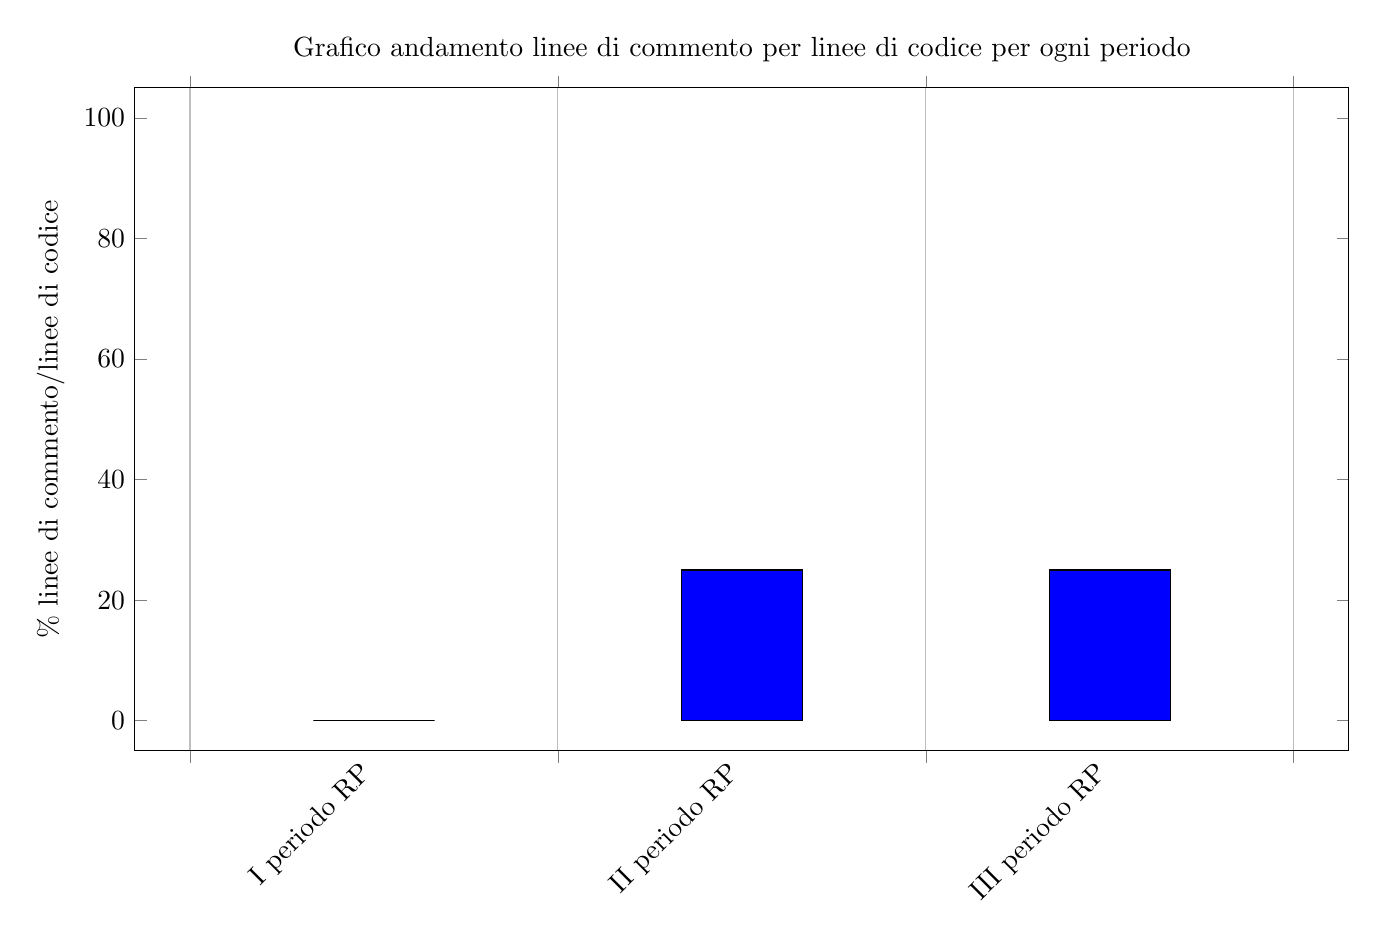
\begin{tikzpicture}

\begin{axis}[
title=Grafico andamento linee di commento per linee di codice per ogni periodo,
x tick label style={
/pgf/number format/1000 sep=},
ylabel=\% linee di commento/linee di codice,
enlargelimits=0.05,
legend style={at={(0.5,-0.4)},
anchor=north,legend columns=-1},
ybar interval=0.33,
symbolic x coords={I periodo RP, II periodo RP, III periodo RP, tmp},%lasciare tmp come ultima colonna per poter visualizzare tutte le colonne tranne tmp
x tick label style={rotate=45,anchor=east},
xtick=data
]
\addplot[fill=blue] coordinates
{(I periodo RP, 0) (II periodo RP, 25) (III periodo RP, 25) (tmp, 100)};

\end{axis}
\end{tikzpicture}


\rowcolors{2}{grigetto}{white}
\renewcommand{\arraystretch}{1.5}
\centering
\begin{longtable}{C{4cm} C{1cm} C{1cm} C{1cm} C{1cm}}
\caption{Elenco degli indici di Gulpease }\\
\rowcolor{darkblue}
\textcolor{white}{\textbf{Documento}} & \textcolor{white}{\textbf{RR}} &
\textcolor{white}{\textbf{RP}} & \textcolor{white}{\textbf{RQ}} & 
\textcolor{white}{\textbf{RA}} \\
\hline
\endhead
\AdRv{1.0.0} & \textcolor{verde}{\textbf{95}} & - & - & -\\
\PdPv{1.0.0} & \textcolor{verde}{\textbf{100}} & - & - & -\\
\PdQv{1.0.0} & \textcolor{verde}{\textbf{100}} & - & - & - \\

\NdPv{1.0.0} & \textcolor{giallo}{\textbf{75}} & - & - & -\\
\SdFv{1.0.0} & \textcolor{verde}{\textbf{94}} & - & - & -\\

\Glossariov{1.0.0} & \textcolor{giallo}{\textbf{67}} & - & - & -\\

Media verbali interni & \textcolor{verde}{\textbf{92}} & - & - & -\\
Media verbali esterni & \textcolor{giallo}{\textbf{65}} & - & - & -\\

\end{longtable}

%\begin{figure}[h]
%	\centering
%	\includegraphics[scale=0.50]{Sezioni/Immagini/IG-Grafico.png}
%	\caption{Grafico andamento dell'Indice di Gulpease per ogni periodo e documento}
%\end{figure}
%}

\pgfplotsset{width=17cm, height=10cm}
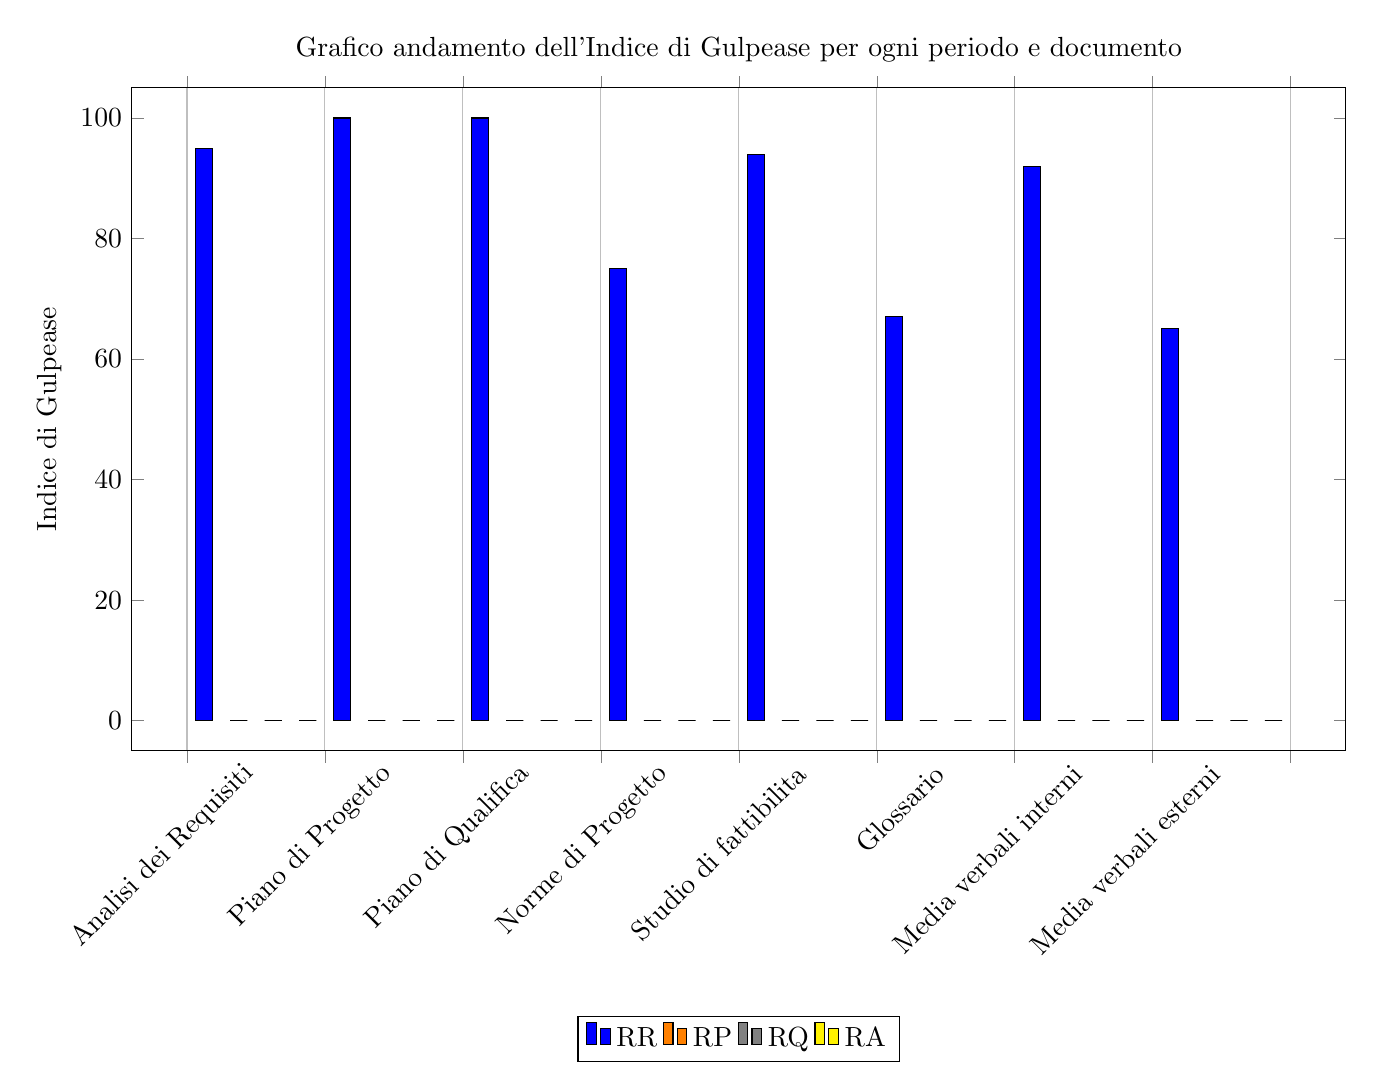
\begin{tikzpicture}

\begin{axis}[
title=Grafico andamento dell'Indice di Gulpease per ogni periodo e documento,
x tick label style={
/pgf/number format/1000 sep=},
ylabel=Indice di Gulpease,
enlargelimits=0.05,
legend style={at={(0.5,-0.4)},
anchor=north,legend columns=-1},
ybar interval=0.5,
symbolic x coords={Analisi dei Requisiti, Piano di Progetto, Piano di Qualifica, Norme di Progetto, Studio di fattibilita, Glossario,
Media verbali interni, Media verbali esterni, tmp},%lasciare tmp come ultima colonna per poter visualizzare tutte le colonne tranne tmp
x tick label style={rotate=45,anchor=east},
xtick=data
]
\addplot[fill=blue] coordinates
{(Analisi dei Requisiti, 95) (Piano di Progetto, 100) (Piano di Qualifica, 100) 
(Norme di Progetto, 75) (Studio di fattibilita, 94) (Glossario, 67)
(Media verbali interni, 92) (Media verbali esterni, 65) (tmp, 0)};

\addplot [fill=orange] coordinates
{(Analisi dei Requisiti, 0) (Piano di Progetto, 0) (Piano di Qualifica, 0) 
(Norme di Progetto, 0) (Studio di fattibilita, 0) (Glossario, 0)
(Media verbali interni, 0) (Media verbali esterni, 0) (tmp, 0)};

\addplot [fill=gray] coordinates
{(Analisi dei Requisiti, 0) (Piano di Progetto, 0) (Piano di Qualifica, 0) 
(Norme di Progetto, 0) (Studio di fattibilita, 0) (Glossario, 0) 
(Media verbali interni, 0) (Media verbali esterni, 0) (tmp, 0)};
\addplot [fill=yellow] coordinates
{(Analisi dei Requisiti, 0) (Piano di Progetto, 0) (Piano di Qualifica, 0) 
(Norme di Progetto, 0) (Studio di fattibilita, 0) (Glossario, 0)
(Media verbali interni, 0) (Media verbali esterni, 0) (tmp, 0)};

\legend{
RR,
RP,
RQ,
RA
}
\end{axis}
\end{tikzpicture}